
% TODO2. ここで入れるべきかわからないが軌跡を導出して補正するというアプローチ自体が新しい
% 一般的な位置推定は軌跡を出してそれを全体最適化というアプローチをとらないきがする
% その点が新しいかもしれない

% TODO: この辺がおかしいので修正: 要修正
\section{目的とアプローチ}

% TODO: 概要図と説明があってないんだよね:要修正
本研究は,様々な環境や状況に対応できるPDRベースの3次元屋内位置推定ライブラリの開発を目的とする.
本研究の概要を図\ref{fig:overview}に示す.
本研究では,PDRを基盤としつつ利用可能な環境情報に応じて適切なアルゴリズムを組み合わせられる柔軟なフレームワークの提供,
環境条件の変化と3次元空間での移動に対応可能な補正アルゴリズム群の実装,
そして実装者が個々の利用環境に最適化された位置推定システムを容易に構築できる直感的なAPIの設計を目指す.
特に複数階層を持つ建物内での継続的な位置推定を実現するため,水平方向の位置推定に加えて,
階層判定を含む垂直方向の移動推定も考慮する.

これらの目的を達成するために,本研究では複数のアプローチを採用する.
第一のアプローチとしてPDRを基盤技術として採用し,その基本機能を独立性の高いコンポーネントとして設計する.
PDRは追加のインフラ整備を必要としない特徴があり,3次元空間を含む様々な環境における位置推定の基盤として適している.
これによって環境条件や要求精度に応じた柔軟な機能選択を実現する.

第二に環境情報を活用した段階的な補正アプローチを導入する.
このアプローチでは,利用可能な環境情報に応じて適切な補正手法を選択・適用する.
例えばフロアマップが利用可能な環境では物理的な移動制約を考慮した補正を行い,
気圧センサーのデータが利用可能な場合は階層判定による垂直方向の移動推定を行う.
これによって様々な環境条件に対応した3次元位置推定の実現を目指す.

第三に拡張性と再利用性を重視したソフトウェアアーキテクチャを採用する.
これにより新たな補正アルゴリズムの追加や,既存アルゴリズムの組み合わせを容易にし,
環境条件の変化への柔軟な対応を可能とする.
また実装者が直感的に理解・使用できるインターフェースを提供し
個々の利用環境に最適化された位置推定システムの構築を支援する.

このように本研究で提案するライブラリは,環境条件に応じて
適切な手法を選択・組み合わせて,
3次元空間における様々な状況に適応可能な屋内位置推定を実現する.
また新たなアルゴリズムやセンサー情報の追加にも柔軟に対応できる拡張性を備え,将来的な技術発展にも対応可能な基盤を提供する.


% TODO:この図修正したいな
\begin{figure}[h]
	\centering
	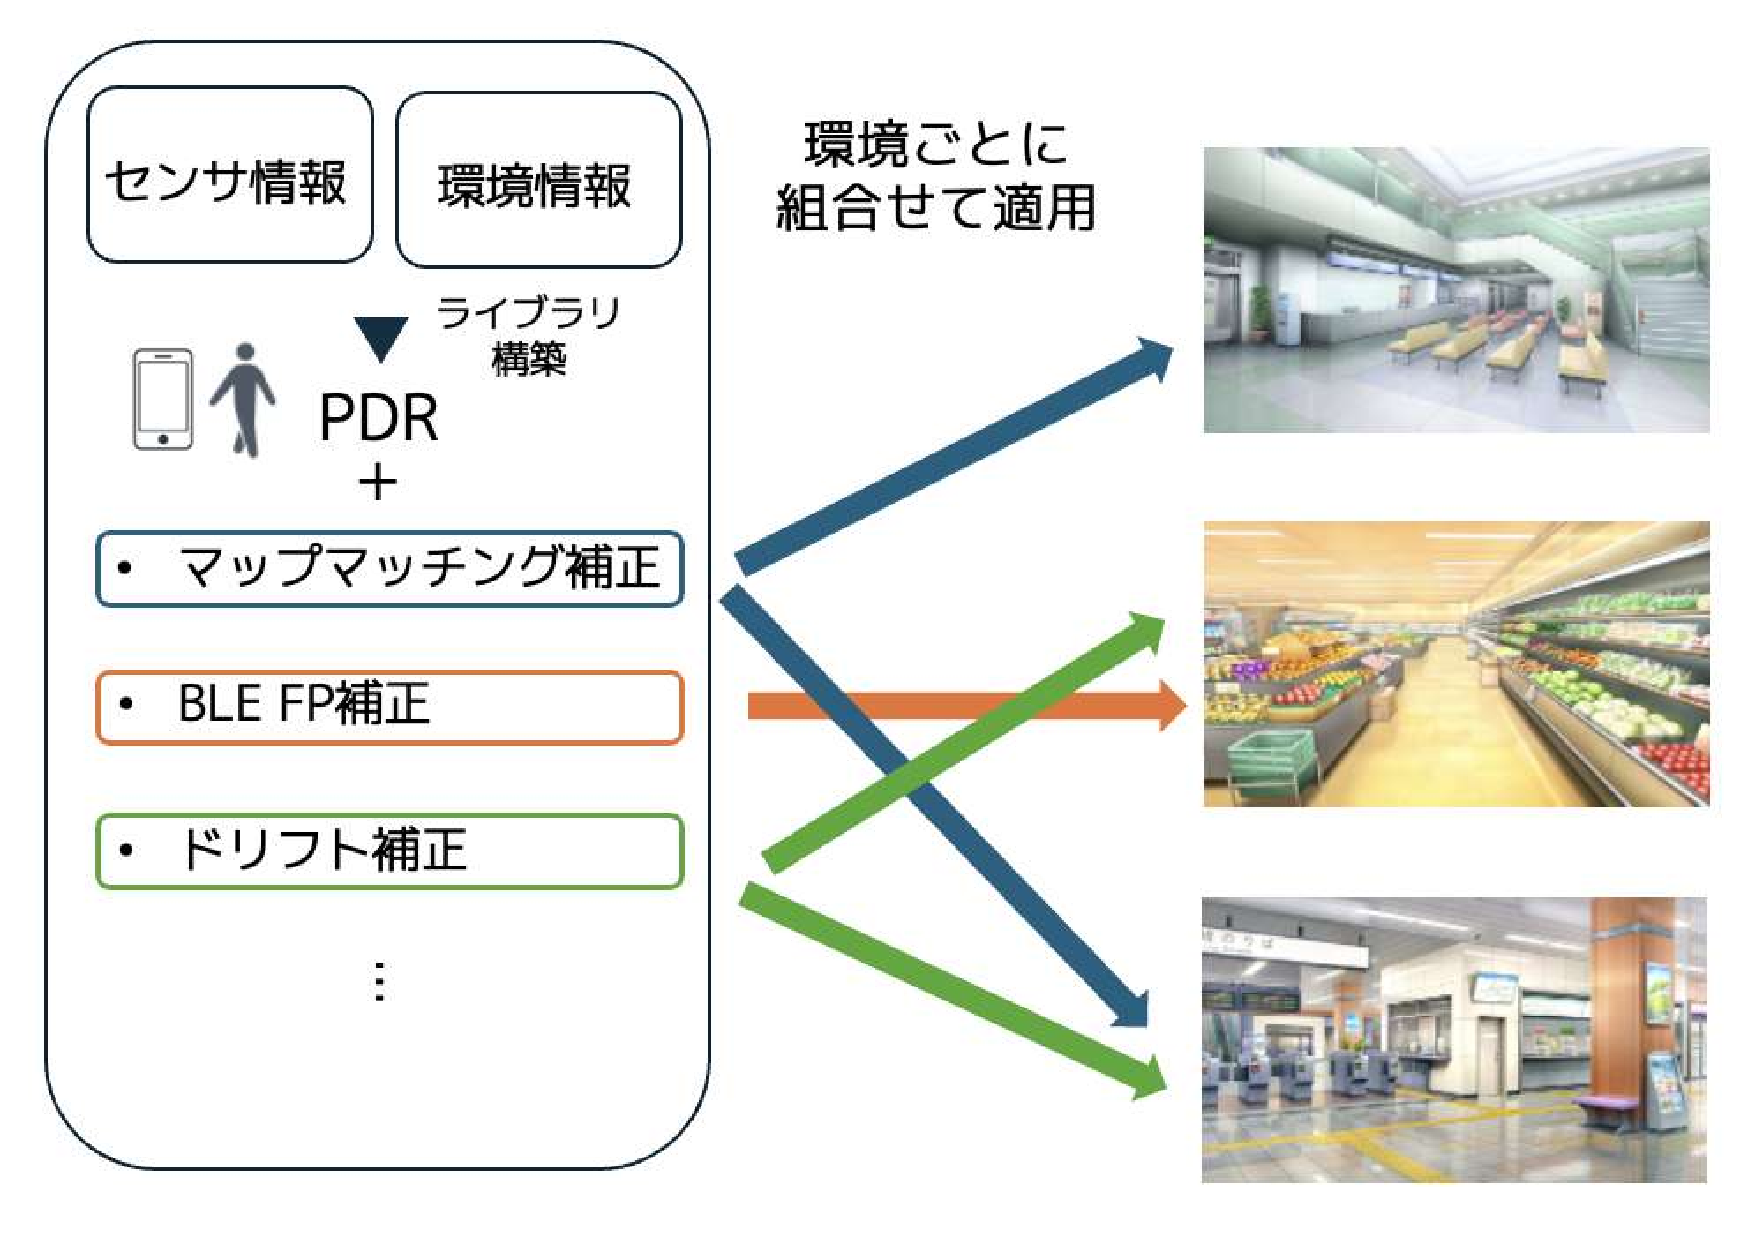
\includegraphics[width=\linewidth]{../image/first.pdf}
	\caption{様々な環境や状況に対応できるPDRベースの\\3次元屋内位置推定ライブラリの概要}    \label{fig:overview}
\end{figure}
